\section{Nonlinear Models}
\paragraph{Primary Text Reading.} \citeA[chap. 4]{tsay2005aft}\index{Tsay, Ruey} and, \citeA{franses2000nlts}
\subsection{Simple Nonlinear Models}

Nonlinear data exists in \fts{}, especially in volatility and high-frequency data. We focus now on simple nonlinear models and neural networks. 

\paragraph{Bilinear Model.} A way to include rate-change points or other nonlinear events is to use a bilinear model such as
\begin{equation}
x_t = c+ \sum^p_{i=1} \phi_i x_{t-i} - \sum^q_{j=1} \theta_j a_{t-j} + \sum^m_{i=1} \sum^s_{j=1} \beta_{ij} x_{t-i} a_{t-j} + a_t,
\label{eq:bilinear}
\end{equation}
where $p,q,m,$ and $s$ are non-negative integers.

Some properties of bilinear models allow the modeling of nonlinear phenomenon with a minimum of parameters. 

\subsubsection{Threshold Autoregressive Model}\label{tar-model}\index{threshold autoregressive\\(TAR) model} Adding some asymmetry to \eqref{eq:bilinear}, we have the threshold autoregressive model, which is a piecewise linear model in the threshold space. For example, a 2-regime AR(1) model 
\[
x_t =
\begin{cases}
-1.5x_{t-1} + a_t, &\text{if $x_{t-1}<0$,} \\
\phantom{-}0.5x_{t-1} + a_t, &\text{if $x_{t-1} \ge 0$,}
\end{cases}
\]
where the $a_{t}$'s are iid\index{iid -- independent and\\identically distributed} $N(0, 1)$. 

Here the delay is 1 time period, $x_{t-1}$ is the threshold variable, and 
the threshold is 0. The threshold divides the $x_{t-1}$ space into two 
regimes with Regime 1 denoting $x_{t-1} < 0$.
% What is so special about this model? See the time plot in Tsay Figure 4.1. 

Special features of this model are,  (a) asymmetry in rising and declining 
patterns, (\textit{more observations are positive than are negative}) (b) the mean of $x_t$ is not zero even though there is no constant term in the model, and (c) the lag-1 coefficient may be greater than 1 in absolute value.

\subsubsection{Markov Switching Model}\index{Markov autoregressive\\switching (MSA) model}
Another example of a two-regime model, but with aperiodic switching is a two-state \emph{Markov autoregressive switching} (MSA) model is
\begin{equation}
x_t = 
\begin{cases}
c_1 + \sum^p_{i=1} \phi_{1,i} x_{t-i} + a_{1t}, &\text{if $s_t=1$,} \\
c_2 + \sum^p_{i=1} \phi_{2,i} x_{t-i} + a_{2t}, &\text{if $s_t=2$,}
\end{cases}
\end{equation} 
where $s_t$ assumes values in $\{1,2\}$ and is a first-order Markov chain 
with transition probabilities,
$P(s_t=2|s_{t-1}=1)=w_1, \quad P(s_t=1|s_{t-1}=2)=w_2,$
and where 0 $\le w_1 \le 1$ is the probability of switching out State 1 from 
time $t-1$ to time $t$. A large $w_1$ means that it is easy to switch out 
State 1, that is, it cannot stay in State 1 for long. The inverse, $1/w_1$, is 
the expected duration (\textit{number of time periods}) to stay in State 1. A similar idea applies to $w_2$. 

% TODO: Example See Figure 4.4 of the textbook (p.166)
% A good source is \citeA{franses2000nlts}.


\subsubsection{Nonparametric Methods}
There may be times when obtaining adequate information about the distribution will be impossible. In that case, we must rely upon nonparametric methods to perform estimation. They are very data dependent and may lead to over fitting of a model.

\margincomment{Kernel density estimators \emph{discover} the data's distribution.}
A major element of nonparametric methods is \emph{smoothing}. To do this, we need a density estimator, which is the construction of an estimate, based on observed data, of an unobservable underlying probability density function. The unobservable density function is thought of as the density according to which a large population is distributed; the data are usually thought of as a random sample from that population.

Using MATLAB functions, kernel density estimation is implemented through the \texttt{ksdensity}\index{ksdensity@\texttt{ksdensity} (in MATLAB)} function. The R language can perform this estimation using \texttt{density}\index{density@\texttt{density} (in R)} function and the \texttt{kde2d} function, for two-dimensional kernel density estimation.

\paragraph{Kernel Regression.} Kernel regression is a non-parametric method to estimate the conditional expectation of a random variable. Its objective is to find a non-linear relationship between two random variables $x$ and $y$, such that
\[
E(y | x) = f(x)
\]
where $f$ is a non-parametric function. The relationship may also be expressed
\[
E(y | x) = \int y f(y|x) dy = \int y \frac{f(x,y)}{f(x)} dy.
\]
A common method is the Nadaraya-Watson kernel regression\index{Nadaraya-Watson kernel regression}, which is an estimate $m$ of a locally weighted average, using a kernel as a weighting function
\[
\widehat{m}(x)=\frac{\sum_{t=1}^T K_h(x-x_t)y_t }{\sum_{t=1}^T K_h(x-x_t)}.
\]

\subsubsection{Neural Networks}\index{neural networks}
Neural networks are non-linear statistical data modeling tools, often used to model complex relationships between inputs and outputs or to find meaningful patterns in data. Because of this, a neural network is a semi-parametric approach to data analysis. Neural networks learn by example. The analyst gathers representative data, and then invokes training algorithms to automatically learn the structure of the data. An example of a neural network is depicted in Figure~\ref{figure:neural-net}. It has a network structure having,
\begin{itemize}
\item Input layer -- This is the observed data that we are trying to discover a relationship to. The aim is to find how known inputs and possibly known outputs are related.
\item Hidden layer -- The relationships between value pairs and the weights applied to them. Since the relationships may be complex, and be linked many ways through \emph{nodes}, there may multiple hidden layers. Sometimes, hidden layer is referred to in data mining literature as both a singular layer and as all layers collectively.
\item Nodes -- The mechanism that links layers together. Some neural network will have multiple hidden layers, and the way their layers are linked (through their nodes) will determine redundancy and search efficiency.
\item Output layer -- The resulting pairing from the input layer that have been paired through the hidden layer. Often, the analyst is uncertain how the pairing occurred, which runs the risk that out-of-sample data may behave differently, and thus, create a different hidden layer with different weightings.
\end{itemize}
The \emph{activation function}, which starts the network, is a logistic function,
\begin{equation}
\ell(z) = \frac{\exp(z)}{1+\exp(z)}
\label{eq:logistic}
\end{equation}
This function is plotted in Figure~\ref{figure:logistic} subject to $[-5,5]$.
\begin{figure}[tb]
	\centering
	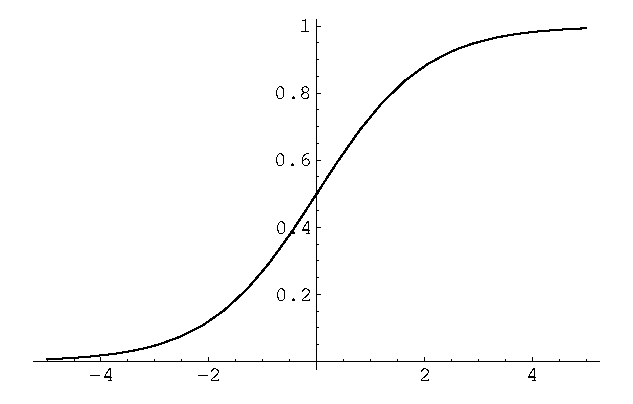
\includegraphics[scale=.8]{logistic}
	\caption{Plot of logistic function in \eqref{eq:logistic}}
	\label{figure:logistic}
\end{figure}
Next, the network requires the Heaviside (or threshold) function, which allows switching between regimes,
\[
H(z)=
\begin{cases}
1 &\text{if $z>0$,} \\
0 &\text{if $z \le 0$.}
\end{cases}
\]

\begin{figure}[tb]
	\centering
	\includegraphics[scale=.5]{neural-net}
	\caption{Example of a neural network}
	\label{figure:neural-net}
\end{figure}

A neural network having a hidden node works through,
\[
x_j = f_j(\alpha_j + \sum_{i \to j} w_{ij} x_i)
\]
where $f_j(\cdot)$ is an activation function which is typically taken to be 
the logistic function \eqref{eq:logistic}. Then, $\alpha_j$ is called the \emph{bias}, the summation $i \to j$ means summing over all input nodes feeding to $j$, and $w_{ij}$ are the weights.
The output node, 
\[
y=f_o(\alpha_o + \sum_{j \to o} w_{jo} x_j),
\]
where the activation function $f_o(\cdot)$ is either linear or a Heaviside 
function. By a Heaviside function, we mean $f_o(z) = 1$ if $z > 0$ and $f_o(z) = 0$, otherwise. Thus, the general form is,
\begin{equation}
y= f_o \Biggr[a_o + \sum_{j \to o} w_{jo} f_j \large( \alpha_j + \sum_{i \to j} w_{ij} x_i \large) \Biggr]
\end{equation}

\paragraph{Supervised Learning.} The task of knowledge discovery in databases (KDD)\index{knowledge discovery\\in databases (KDD)} allows the analyst to examine data and its relationship to functional forms in two ways. The first, is through \emph{supervised learning}.  We have a set of data pairs $(x, y)$, $x \in X$, $y \in Y$ and the goal is to find a function $f$ within a class of functions that relates to the pairs. This ``supervised'' method requires us to infer how the mapping implied by the data and the cost function is related to the mismatch between our mapping and the data.

\paragraph{Unsupervised Learning.} By contrast, through \emph{unsupervised learning} we are given some data $x$, and a cost function $c(\cdot)$ which is minimized with respect to any function of $x$ and the network's output, $f$. The cost function is determined by the task formulation. In this method, we have little, if any, idea how the data are related. We let the data make the connection for us.

\paragraph{Training and Forecasting.} Divide the data into training and forecasting subsamples. In the training subsample, build a few network systems. The forecasting is based on the accuracy of out-of-sample forecasts to select the ``best'' network. 

\subsection{Complex Nonlinear Models}\label{spectral methods}
\subsubsection{Cosine Seasonality}\index{spectral methods}
In some markets, seasonal energy markets, for instance, there may be at least two seasonal factors \cite{pilipovic2007er}\index{Pilipovic, Dragana}.
\margincomment[red]{These are examples of two-regime models.}
The cosine function can capture these factors, requiring relatively few parameters -- the magnitude of the seasonal factor, and the time of year when it occurs. Here is a function that capture two different periodicities,

\begin{equation}
\index{beta@$\beta$ (beta)!in regression}
\overbrace{\beta_1 \cos(2 \pi (T-t^C_1))}^{annual} + \underbrace{\beta_2 \cos(4 \pi(T-t^C_2))}_{semi-annual}
\label{eq:cos-season}
\end{equation}
We can model two different seasonal patterns in \eqref{eq:cos-season} by representing $t^C_1$ with $\beta_1$ magnitude, as the annual center, and $t^C_2$ with $\beta_2$ magnitude, as the semi-annual center.

\subsubsection{Exponential Seasonality}
Using repetitive exponential functions is another way to model seasonality to capture a more narrow rise and fall of the \fts{}. This is different from the cosine function, in which the seasonal factor affects the entire curve. With exponential seasonality, we can apply local treatment,
\begin{equation}
\beta_1 \exp\Big({-\gamma_1 \big(rfc(T-t^C_1)\big)^2} \Big)+ \beta_2 \exp\Big({-\gamma_2 \big(rfc(T-t^C_2)\big)^2} \Big),
\label{eq:exp-season}
\end{equation}
where the function $rfc$ is annually repetitive, and returns the annualized time to or from the closest center $t^C_i$ for seasonal factor $i$. The two seasonal factors in \eqref{eq:exp-season} each has a center at $t^C$, a magnitude $\beta$\index{beta@$\beta$ (beta)!in regression}, and a width of the seasonal peak defined by the ``decay'' coefficient $\gamma$.

%\subsection{Nonlinearity Testing}

%\subsubsection{Nonparametric Tests}

%\subsubsection{Parametric Tests}

%\subsection{Forecasting}
